\chapter{INTRODUCTION}
To provide learning resources, educational institutions use online learning platforms. Students can engage in learning activities and communicate with one another using these technologies. Distant web locations. Security risks are raised by this behavior. Additionally, worries about the validity of the online test procedure have grown, which is one of activities that are essential for online learning \cite{rosmansyah2020impersonation}.


Technological advancements are rendering traditional digital forensics techniques and tools potentially obsolete. Proactive approaches, emphasizing remote investigation capabilities, are emerging as a new paradigm to address this challenge. \citet{machaka2022InvestigatingProactiveDigitalForensicsLeveragingAdversaryEmulation}. Digital forensics underpins effective cybersecurity incident response. Its methods enable reconstruction of attack sequences, providing a clear understanding of malicious actions. This forensic analysis empowers responders to contain threats and implement mitigation strategies, while also potentially yielding legally valuable evidence\citet{johansen2017Digitalforensicsandincidentresponse}. 

The continuous advancement of information technology has witnessed a surge in the adoption of electronic examination (e-exam) systems by researchers and organizations. Concurring with prior research \citet{al2017efficienteexamscheme}, institutions employing e-exam systems must prioritize robust security measures. These safeguards are paramount for ensuring the confidentiality, integrity, and availability of examination information, ultimately protecting the institution's reputation. One method for gathering logs indicative of online exam cheating is by utilizing log management.

In "Guide to Computer Security Log Management," NIST Special Publication 800-92, a thorough framework for creating and sustaining efficient log management procedures is presented. Given that it describes methods for gathering, examining, and maintaining digital evidence, this approach is especially pertinent to tackling the problems associated with online exam cheating.

Reactive forensics, which investigates incidents post-occurrence, poses significant risks in addressing online exam threats. Delayed detection can lead to greater damage to exam integrity and institutional reputation, along with the potential loss of critical evidence, such as deleted log data. This approach is not only resource-heavy, demanding extensive time and effort, but also lacks preventive capabilities, allowing misconduct to persist. As online exam platforms grow, reactive methods may struggle to manage the increasing volume of data and incidents effectively.

In order to solve these problems, proactive forensics uses anomaly detection, log management, and real-time monitoring to spot dangers as they materialize. The security and integrity of online tests are guaranteed by frameworks such as NIST 800-92, which allow institutions to quickly identify and prevent evidence data loss.

The purpose of this research is to explore the application of proactive forensic techniques, guided by NIST 800-92, in addressing challenges such as cheating and system abuse in online exam systems. By integrating log management with real-time anomaly detection, this study aims to enhance the security, reliability, and integrity of e-exams, offering practical solutions for modern educational institutions.

\section{Rationale}

%The growing usage of Learning Management Systems (LMS) in training and education has made the problem of cheating on online tests more pertinent. Participants benefit from increased flexibility and accessibility while taking exams online, but maintaining exam integrity also becomes more difficult. Consequently, it is crucial in this situation to apply proactive forensics using a log management strategy.
%Given the complexity of today's fraud problems, a reactive approach for cheating detection where analysis is done after an incident has happened is no longer enough. Because proactive forensics can identify suspicious activity in real time, it provides a more sophisticated solution that enables institutions to take action before cheating happens.
The adoption of Learning Management Systems (LMS) in Indonesia has grown rapidly in recent years, especially accelerated by the COVID-19 pandemic. According to a recent report, internet penetration in Indonesia exceeded 77\% in early 2024, providing a strong foundation for the widespread use of online learning platforms \cite{intimedia2024}. In fact, secondary schools have been found to utilize LMS tools almost twice as much as universities, making them the most dominant sector in formal education for LMS adoption \cite{akubelajar2024}.

Empirical studies also indicate that LMS usage significantly improves student learning outcomes in Indonesia. For example, research at the primary school level found that LMS contributed to 46.7\% of the variance in student performance (R$^2$ = 0.467) \cite{ucy2023}. Despite these advantages, challenges remain—such as limited student engagement and insufficient technical support in some institutions \cite{edukatif2023}.

Given this rapid expansion and the projected value of the Indonesian online education platform market, which is estimated to reach IDR 60 trillion by 2029 \cite{tracedata2024}, ensuring the security and integrity of online examination systems through proactive forensic log management has become an urgent priority.

\begin{figure}[htbp]
	\centering
	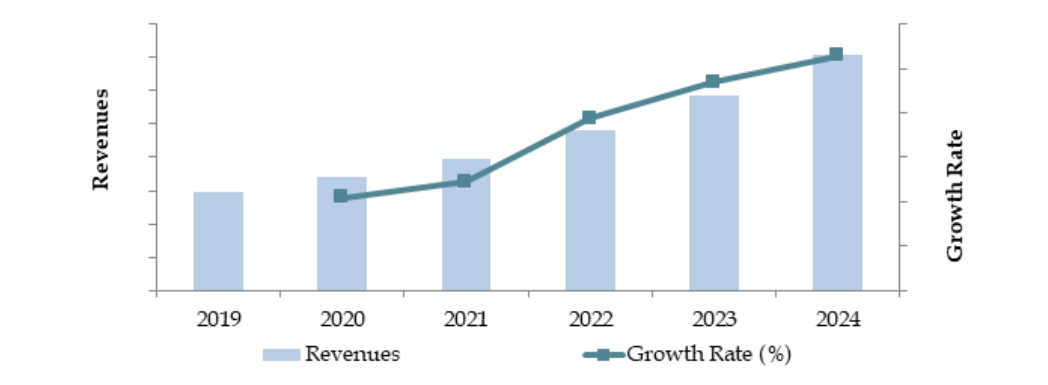
\includegraphics[width=0.7\textwidth]{figure/indonesia-online-platform-market.png}
	\caption{Market Size and Growth Rate of Indonesia Online Education Platforms (2019--2024) \cite{tracedata2024}.}
	\label{fig:market-growth}
\end{figure}

The widespread adoption of Learning Management Systems (LMS) in Indonesia has transformed the way educational institutions deliver instruction and assess student learning. As a result, crucial academic activities such as examinations, assignments, and student-instructor interactions are now conducted and recorded digitally within these platforms.

However, the shift to digital learning environments introduces new challenges, especially in maintaining exam integrity and institutional reputation. In this context, the role of comprehensive log management becomes paramount. Every action within the LMS generates digital traces (logs), which, if systematically collected, stored, and analyzed, can serve as crucial evidence in detecting academic misconduct, troubleshooting system issues, and ensuring compliance with institutional policies.

Without a robust log management strategy, institutions risk losing critical information that could be vital for investigating suspicious activities or resolving disputes. Therefore, as LMS usage continues to expand, the need for effective and proactive log management frameworks becomes an essential component of educational quality assurance and digital forensic readiness.

Despite the numerous benefits brought by online learning, real-world incidents have highlighted the critical risks of poor log management. For instance, several Indonesian universities reported difficulties in investigating alleged cheating during high-stakes online exams due to missing or incomplete log data, which hampered both technical and legal resolution of the cases \cite{rosmansyah2019attackdefensetreeonaeexamsystem, lintang2024log}. These incidents underscore that without a robust, centralized, and proactive log management strategy, institutions not only risk losing vital forensic evidence but may also face reputational and regulatory consequences.

Effective log management does not merely support post-incident investigation; it also enables institutions to fulfill compliance obligations, reduce the time required for incident response, and foster greater trust among students, faculty, and accreditation bodies \cite{rivera2019towards, abd2024enhancing}.
% =========================================================
\section{Theoretical Framework}

This research adopts a theoretical foundation grounded in the principles of digital forensics, information security, and structured log management. The primary reference is the NIST Special Publication 800-92, which outlines the log management lifecycle comprising log generation, collection, transmission, storage, analysis, preservation, and reporting \cite{kentnist800922006guide}. This framework ensures the integrity, availability, and traceability of digital evidence in online systems.

Digital forensics theory, as defined by McKemmish and subsequent researchers, emphasizes the systematic identification, preservation, analysis, and presentation of digital evidence \cite{mckemmish1999}. In the context of online examination systems, these principles require that all relevant events—such as user authentication, quiz attempts, and system access—are reliably captured and retained for potential forensic review.

Furthermore, this study integrates contemporary advances in log analysis, specifically the use of machine learning algorithms for anomaly detection. Recent work highlights that unsupervised models, such as Isolation Forests, can effectively identify suspicious behaviors in LMS log data without requiring labeled datasets \cite{garg2023preserving, lintang2024log}.

By combining the log lifecycle model from NIST SP 800-92 with digital forensic readiness principles and modern anomaly detection techniques, the proposed framework aims to provide a proactive and comprehensive solution for ensuring the security, reliability, and integrity of online examination processes.

\section{Conceptual Framework/Paradigm}

Identify and discuss the variables related to the problem, and present a schematic diagram of the paradigm of the research and discuss the relationship of the elements/variables therein.

\section{Statement of the Problem}
The issue of cheating in online exams has become increasingly relevant with the increased use of Learning Management Systems (LMS) in education and training. \citet{ranger2020detection} mention about several indicator of cheating .The use of online exams provides greater flexibility and access to participants, but also creates new challenges in ensuring exam integrity.
 
\begin{enumerate}
    \item Inefficient Log Management Existing log handling methods lack automation and centralization, leading to delays in collection, storage, and analysis, which undermines forensic readiness.
    \item Risk of Evidence Loss Without a robust system for log preservation, critical evidence may be lost or become unreliable, compromising forensic investigations in online examination platforms.
    \item Lack of Alerts and Reporting The absence of integrated alert systems and reporting mechanisms limits timely detection of anomalies and documentation of potential irregularities for further analysis.
\end{enumerate}


\section{Objective and Hypotheses}

\textbf{Objective} 

The actual purpose of the proposed method for log management in proactive forensic systems would be to create a reliable and orderly structure for the acquisition, storing and analysis of log data. The method is likely to increase forensic preparedness by making the log data collection process automated and centralizing it towards a secured place, which will also ensure the integrity and availability of digital evidence and risk of losing data. Using the NIST 800-92 framework for security log management equips organizations with the tools and practices to handle logs effectively. It enhances forensic readiness
\begin{itemize}
    \item Designing and deploying a log management system that centralizes log handling to enable efficient management, secure storage, and preparedness for forensic analysis within an online examination platform.
    \item Developing a system that automates and proactively collects, stores, and analyzes log data to enhance forensic readiness and ensure the availability of critical evidence for investigations.
    \item Incorporating a reporting mechanism to document potential irregularities and 
    support further forensic analysis based on the automated log evaluation process.
\end{itemize}


\textbf{Hypothesis}

\begin{enumerate}
    \item The efficiency and accuracy of log management will be increased by automating and centralizing the collecting of logs from different parts of an online examination platform, such as server logs, user activity logs, and LMS like Moodle. This will allow for better monitoring and the identification of suspicious activity.
    \item Automating the processes of collecting, storing, and analyzing log data enhances forensic readiness by guaranteeing the reliable availability of crucial evidence for efficient and timely investigations.
    \item The impact of security issues is reduced by integrating real-time alert systems, such as Telegram dashboards or notifications, which improve administrators' or proctors' capacity to identify, respond quickly and effectively to anomalies found.
    \item A structured preliminary report for online tests that includes user activity patterns and in-depth log analysis can help identify anomalies and offer practical advice for maintaining the integrity of the test.Forensic investigations and more precise tracking of cheating will be made possible by effective data log management.
\end{enumerate}


\section{Contribution}
Proactive forensic techniques, guided by the NIST 800-92 log management framework, provide a structured and efficient approach to securing and analyzing logs. On purpose evidence data loss for forensically sound
% =========================================================
\section{Assumption}


\begin{enumerate}
    \item Accurate Documentation of Participant Activities: The log system reliably documents all participant activities during the EPT exam.
    \item Authenticity of Preserved Log Data: The log data is trustworthy for examining examinee behavior because it is gathered from trusted sources and hasn't been altered.
    \item Logs Show Real User Behavior: The recorded behavior patterns show the examinees' real activities because the generated log data accurately depicts their actions during the test.
\end{enumerate}
% The following conclusions about English Proficiency Test (EPT) tests using logs as the data source can be drawn:
These presumptions serve as the foundation for proactive forensics research and application in identifying possible irregularities or cheating during online EPT tests.
    

